\subsection{UCG - Caso d'uso generale}
\begin{figure}[H] 
	\centering
	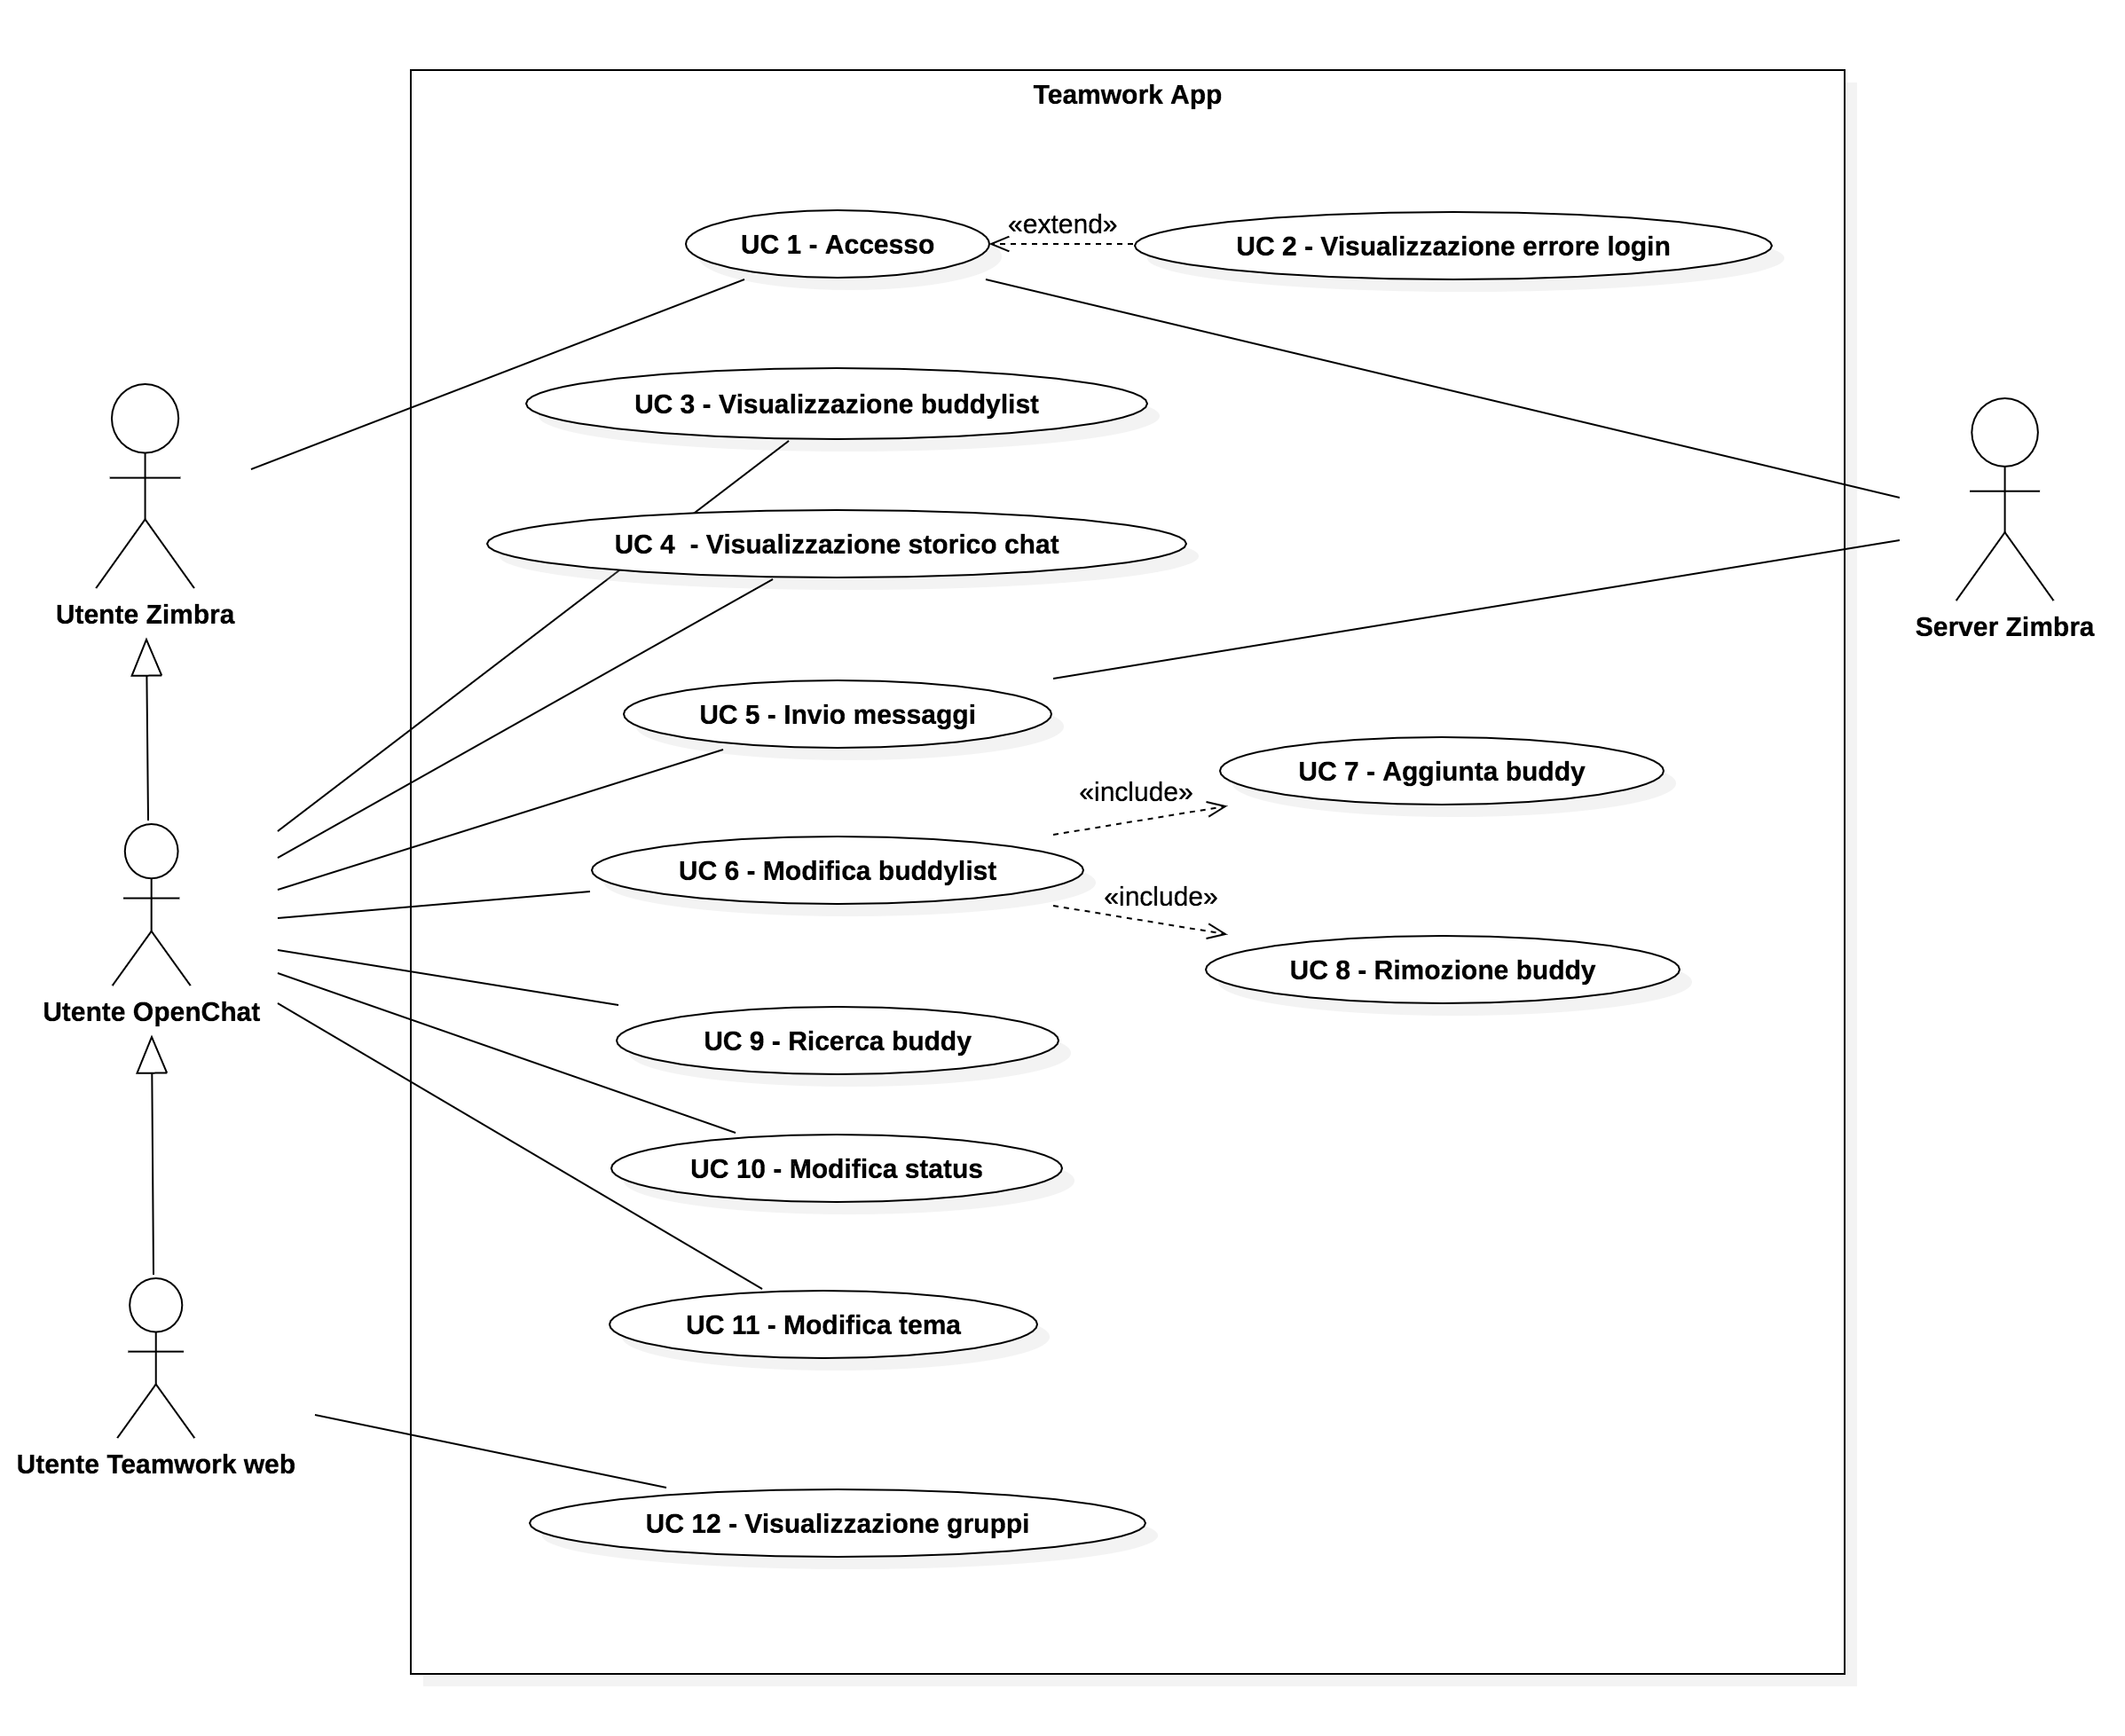
\includegraphics[scale=0.17]{UC/UCG}
	\caption{UCG - Caso d'uso generale}
\end{figure}

% ---------------------------------------------------------------------------- %
\subsection{UC1 - Accesso}
\begin{figure}[H] 
	\centering
	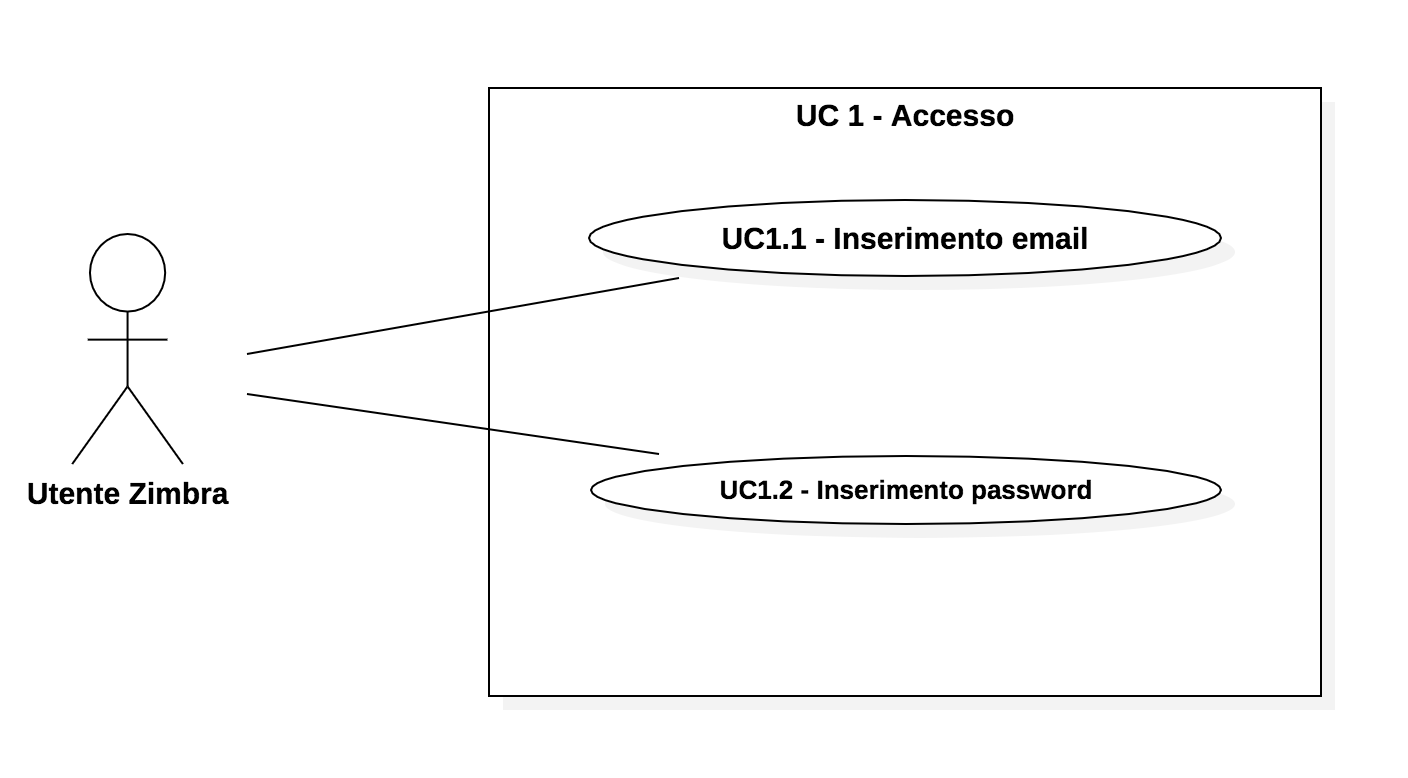
\includegraphics[scale=0.17]{UC/UC1}
	\caption{UC1 - Accesso}
\end{figure}
\begin{center}
	\bgroup
	\def\arraystretch{1.8}     
	\begin{longtable}{  p{4cm} | p{9.5cm} } 
		\textbf{Attori Primari} & Utente Zimbra; \\ 
		\textbf{Descrizione} & L’attore si può autenticare inserendo e-mail e password con cui è registrato al server Zimbra; \\ 
		\textbf{Precondizioni}  & Il sistema è avviato e pronto per l’utilizzo e mostra la pagina di login; \\
		\textbf{Postcondizioni} & Il sistema ha autenticato l’attore e quindi mostra all’attore autenticato la sua area riservata;  \\ 
		\textbf{Scenario principale} & 
			1. L’attore inserisce l'e-mail con cui è registrato al server Zimbra); \newline
			2. L’attore inserisce la sua password; \newline
			3. L’attore conferma il login e accedere alla sua area riservata.\\
		\textbf{Estensioni} & Visualizzazione errore login (riferimento).
	\end{longtable}
	\egroup
\end{center}

% ---------------------------------------------------------------------------- %

\subsection{UC1.1 - Inserimento email}
\subsection{UC1.2 - Inserimento password}

% ---------------------------------------------------------------------------- %

\subsection{UC2 - Visualizzazione errore login}
\begin{center}
	\bgroup
	\def\arraystretch{1.8}     
	\begin{longtable}{  p{4cm} | p{9.5cm} } 
		\textbf{Attori Primari} & Utente Zimbra; \\ 
		\textbf{Descrizione} &  L'attore visualizza un messaggio di errore in quanto le credenziali da lui inserite non sono corrette; \\ 
		\textbf{Precondizioni}  & L'attore ha cercato di effettuare il login inserendo delle credenziali errate; \\
		\textbf{Postcondizioni} & L'attore ha visualizzato il messaggio di errore;  \\ 
		\textbf{Scenario principale} & 
		1. L'attore visualizza il messaggio di errore;
	\end{longtable}
	\egroup
\end{center}

% ---------------------------------------------------------------------------- %

\subsection{UC3 - Visualizzazione buddylist}
\begin{figure}[H] 
	\centering
	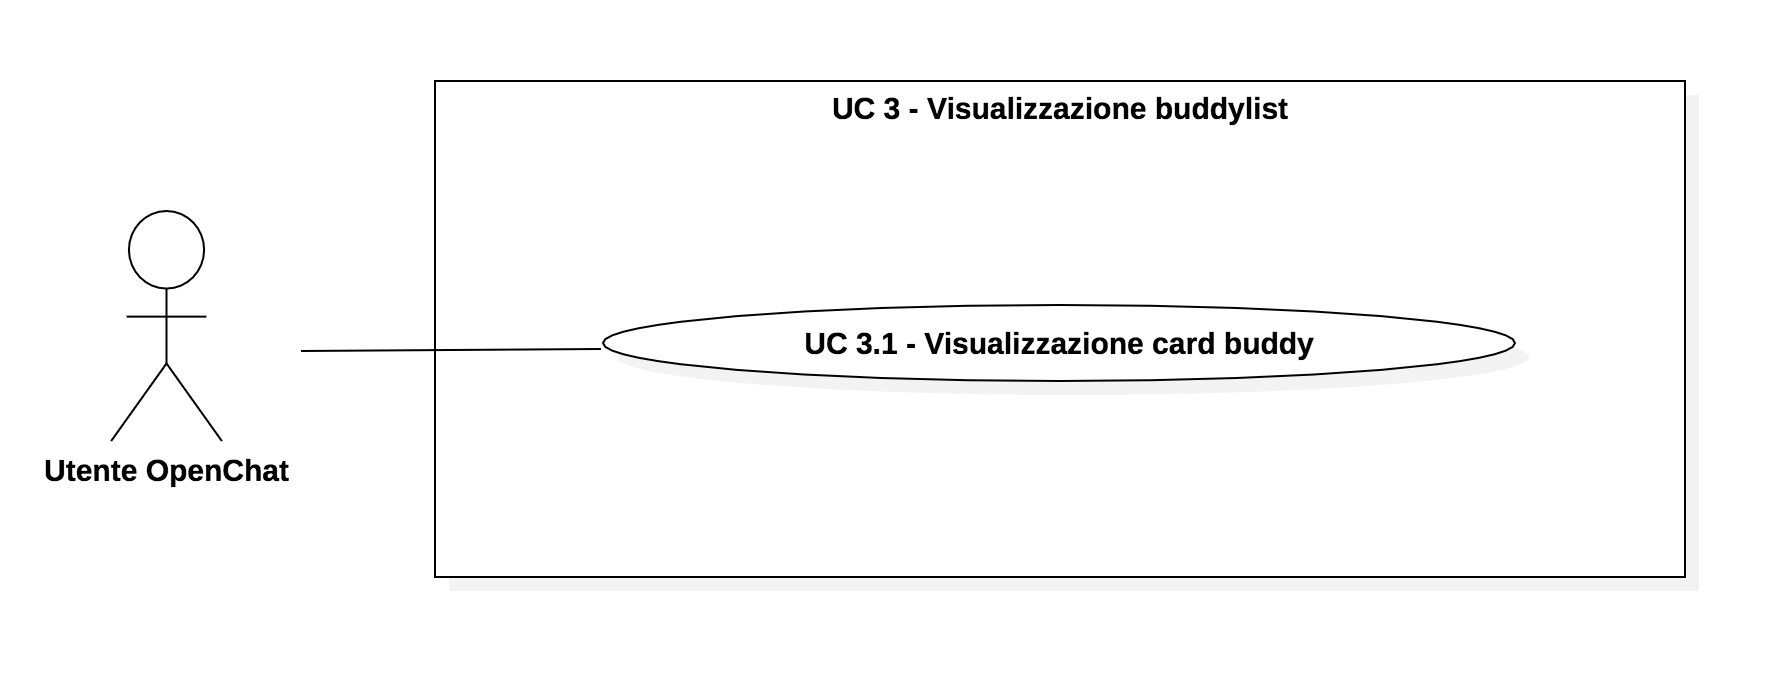
\includegraphics[scale=0.17]{UC/UC3}
	\caption{UC3 - Visualizzazione buddylist}
\end{figure}
\begin{center}
	\bgroup
	\def\arraystretch{1.8}     
	\begin{longtable}{  p{4cm} | p{9.5cm} } 
		\textbf{Attori Primari} & Utente OpenChat; \\ 
		\textbf{Descrizione} &  L'attore può visualizzare l'intera lista dei buddy presenti nella sua buddylist; \\ 
		\textbf{Precondizioni}  & Talkapp presenta all'attore una pagina contenente la lista dei suoi buddy; \\
		\textbf{Postcondizioni} & L'attore ha visualizzato la lista dei suoi buddy;  \\ 
		\textbf{Scenario principale} & 
		1. L'attore seleziona l'icona nella tab riguardante la buddylist; \newline
		2. L'attore visualizza la buddylist contenente tutti i suoi buddy;
	\end{longtable}
	\egroup
\end{center}

\subsection{UC3.1 - Visualizzazione card buddy}
\begin{figure}[H] 
	\centering
	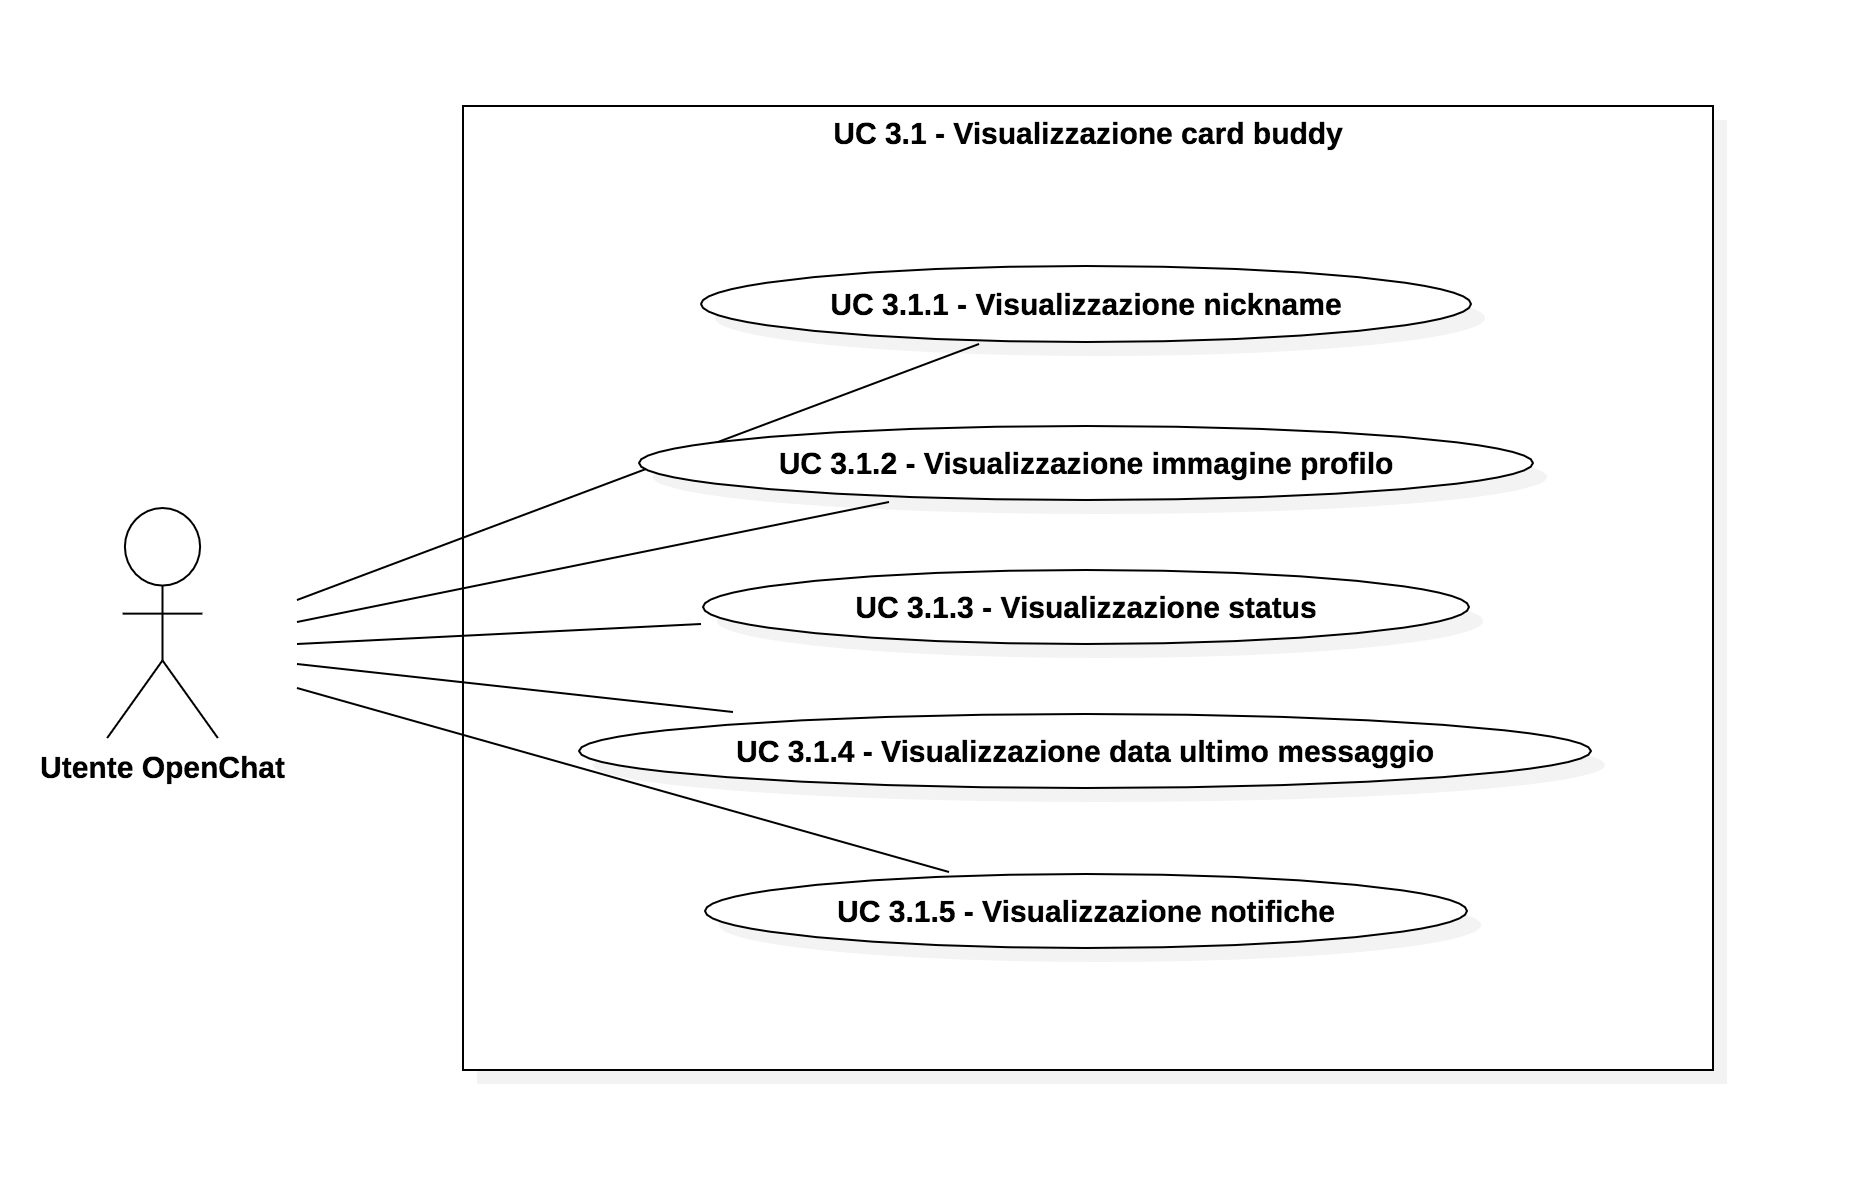
\includegraphics[scale=0.17]{UC/UC3_1}
	\caption{UC3.1 - Visualizzazione card buddy}
\end{figure}

\subsection{UC3.1.1 - Visualizzazione nickname}

\subsection{UC3.1.2 - Visualizzazione immagine profilo}

\subsection{UC3.1.3 - Visualizzazione status}

\subsection{UC3.1.4 - Visualizzazione data ultimo messaggio}

\subsection{UC3.1.5 - Visualizzazione notifiche}

% ---------------------------------------------------------------------------- %

\subsection{UC4 - Visualizzazione storico chat}
\begin{figure}[H] 
	\centering
	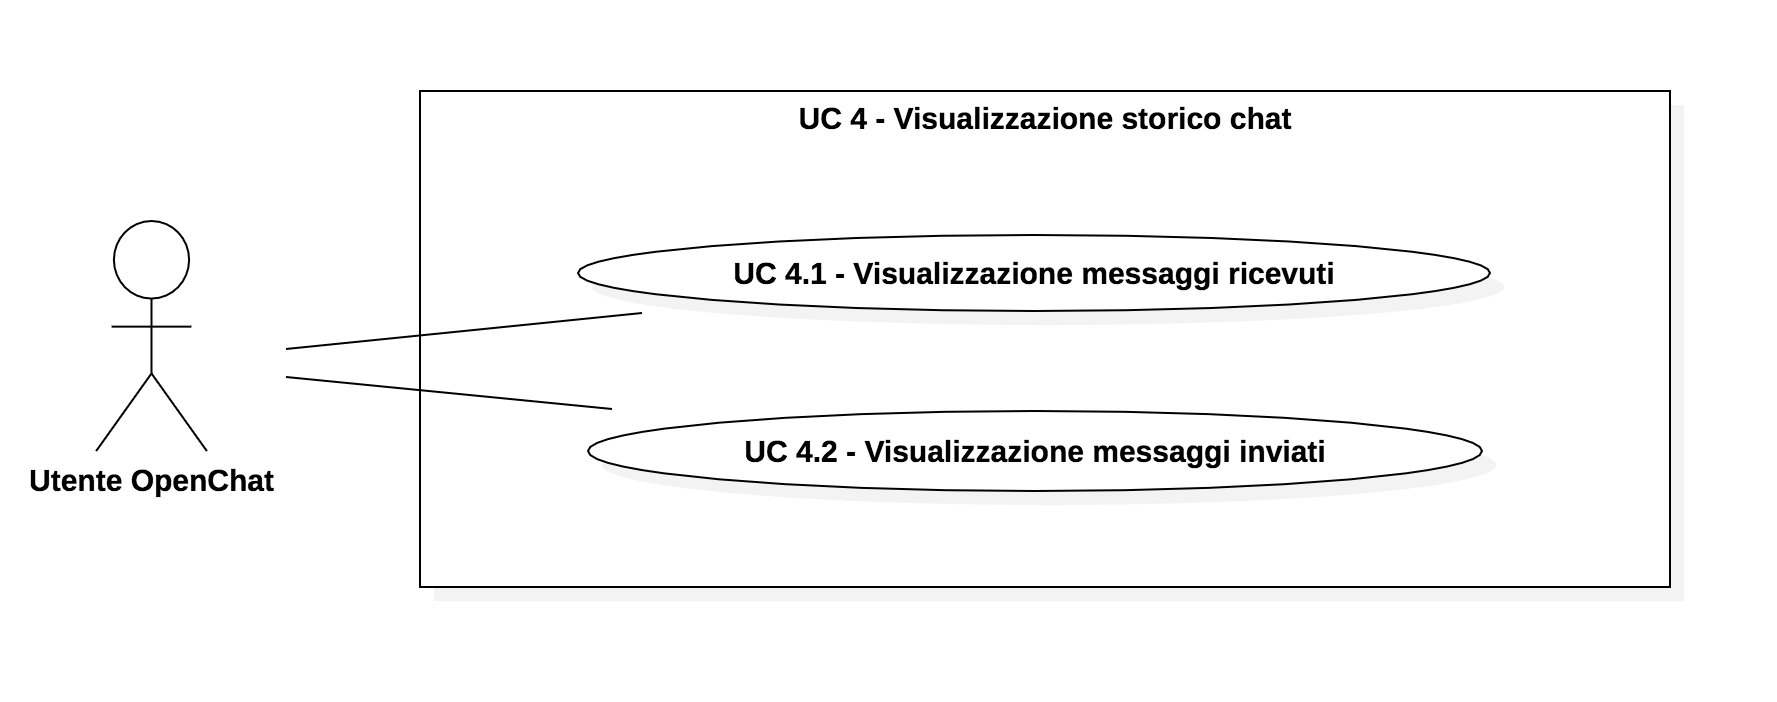
\includegraphics[scale=0.17]{UC/UC4}
	\caption{UC4 - Visualizzazione storico chat}
\end{figure}


\subsection{UC4.1 - Visualizzazione messaggi ricevuti}

\subsection{UC4.2 - Visualizzazione messaggi inviati}


% ---------------------------------------------------------------------------- %

\subsection{UC5 - Invio messaggi}

\subsection{UC6 - Modifica buddylist}

\subsection{UC7 - Aggiunta buddy}
\begin{center}
	\bgroup
	\def\arraystretch{1.8}     
	\begin{longtable}{  p{4cm} | p{9.5cm} } 
		\textbf{Attori Primari} & Utente OpenChat; \\ 
		\textbf{Descrizione} &  L'attore può aggiungere un nuovo buddy alla sua buddylist; \\ 
		\textbf{Precondizioni}  & Talkapp presenta all'attore una pagina contenente un form per l'aggiunta di un buddy; \\
		\textbf{Postcondizioni} & L'attore ha aggiunto un buddy alla sua buddylist;  \\ 
		\textbf{Scenario principale} & 
		1. L'attore inserisce il nickname che vuole dare al buddy; \newline
		2. L'attore inserisce l'e-mail del buddy che vuole aggiungere; \newline
		3. L'attore conferma l'aggiunta del buddy alla propria buddylist.
	\end{longtable}
	\egroup
\end{center}

\subsection{UC8 - Rimozione buddy}
\begin{center}
	\bgroup
	\def\arraystretch{1.8}     
	\begin{longtable}{  p{4cm} | p{9.5cm} } 
		\textbf{Attori Primari} & Utente OpenChat; \\ 
		\textbf{Descrizione} &  L'attore può rimuovere un buddy dalla sua buddylist; \\ 
		\textbf{Precondizioni}  & Talkapp presenta all'attore una pagina contenente i dettagli del buddy selezionato e le azioni che possono essere svolte; \\
		\textbf{Postcondizioni} & L'attore ha rimosso il buddy dalla sua buddylist;  \\ 
		\textbf{Scenario principale} & 
		1. L'attore seleziona il buddiy dalla buddylist che vuole rimuovere; \newline
		2. L'attore seleziona la voce "Rimozione" dal menù di azioni disponibili; \newline
		3. L'attore conferma la rimozione del buddy dalla propria buddylist.
	\end{longtable}
	\egroup
\end{center}

\subsection{UC9 - Ricerca buddy}
\begin{center}
	\bgroup
	\def\arraystretch{1.8}     
	\begin{longtable}{  p{4cm} | p{9.5cm} } 
		\textbf{Attori Primari} & Utente OpenChat; \\ 
		\textbf{Descrizione} &  L'attore può ricercare un  buddy tra quelli presenti nella sua buddylist; \\ 
		\textbf{Precondizioni}  & Talkapp presenta all'attore una pagina contenente un campo di ricerca per ricercare un buddy in base ad un certo testo; \\
		\textbf{Postcondizioni} & L'attore ha ricercato un buddy dalla sua buddylist in base ad un testo da lui inserito;  \\ 
		\textbf{Scenario principale} & 
		1. L'attore inserisce dei caratteri nel campo di ricerca; \newline
		2. L'attore visualizza i buddy corrispondenti alla ricerca da lui effettuata;
	\end{longtable}
	\egroup
\end{center}

\subsection{UC10 - Modifica status}
\begin{center}
	\bgroup
	\def\arraystretch{1.8}     
	\begin{longtable}{  p{4cm} | p{9.5cm} } 
		\textbf{Attori Primari} & Utente OpenChat; \\ 
		\textbf{Descrizione} &  L'attore può modificare lo status con cui viene visualizzato dagli altri utenti; \\ 
		\textbf{Precondizioni}  & Talkapp presenta all'attore una pagina contenente un elenco degli statusdis ponibili; \\
		\textbf{Postcondizioni} & L'attore ha modificato lo status con cui viene visualizzato dagli altri utenti; \\ 
		\textbf{Scenario principale} & 
		1. L'attore seleziona uno status tra quelli disponibili; \newline
		2. L'attore conferma di voler cambiate status con quello selezionato;
	\end{longtable}
	\egroup
\end{center}

\subsection{UC11 - Modifica tema}
\begin{center}
	\bgroup
	\def\arraystretch{1.8}     
	\begin{longtable}{  p{4cm} | p{9.5cm} } 
		\textbf{Attori Primari} & Utente OpenChat; \\ 
		\textbf{Descrizione} &  L'attore può modificare il tema dei colori con cui visualizza l'applicazione; \\ 
		\textbf{Precondizioni}  & Talkapp presenta all'attore una pagina contenente un elenco con tutti i temi disponibili; \\
		\textbf{Postcondizioni} & L'attore ha modificato il tema dell'applicazione; \\ 
		\textbf{Scenario principale} & 
		1. L'attore seleziona un tema tra quelli disponibili da applicare \newline
		2. L'attore conferma di voler applicare quel tema;
	\end{longtable}
	\egroup
\end{center}

\subsection{UC12 - Visualizzazione gruppi}
\begin{center}
	\bgroup
	\def\arraystretch{1.8}     
	\begin{longtable}{  p{4cm} | p{9.5cm} } 
		\textbf{Attori Primari} & Utente Teamwork web; \\ 
		\textbf{Descrizione} &  L'attore può visualizzare l'elenco dei gruppi di cui fa parte; \\ 
		\textbf{Precondizioni}  & Talkapp presenta una pagina contenente i gruppi di cui fa parte; \\
		\textbf{Postcondizioni} & L'attore ha visualizzato i gruppi di cui fa parte; \\ 
		\textbf{Scenario principale} & 
		1. L'attore seleziona l'icona nella tab riguardante i gruppi; \newline
		2. L'attore visualizza i gruppi di cui fa parte;
	\end{longtable}
	\egroup
\end{center}

